\documentclass[11pt]{article}
\usepackage[margin=2.5cm]{geometry}
\usepackage{graphicx,booktabs,hyperref,amsmath}
\usepackage[T1]{fontenc}
\hypersetup{colorlinks=true,linkcolor=black,urlcolor=blue,citecolor=black}
\newcommand{\as}{$''$}
\title{Candidate images of the near-Earth asteroid (1627) Ivar on Harvard plates of 1901, 28 years before its discovery}
\author{Qianghao Wu}
\date{November 28, 2026}
\begin{document}
\sloppy
\maketitle

\begin{abstract}
The earliest observation of the near-Earth asteroid (1627) Ivar in the JPL Small-Body Database and in the Minor Planet Center observation list is its discovery on 1929 Sep 25. We searched public scans of Harvard plates of the bright apparitions of 1901, 1906 and 1929 for it with a test that we registered in advance: the plate rule, the predicted positions, the statistic and the decision rule were committed before any image was downloaded. The rule selected six plates. One plate does not cover the position, and no 1906 plate met the rule. All four measurable plates of 1901, taken at Arequipa from 1901 Jul 18 to 1901 Sep 22, pass the per-plate threshold. The probability of four passes under the per-plate null rates, which come from 300 random regions on each plate, is about $10^{-6}$ ($1.2\times10^{-6}$; $1.8\times10^{-5}$ with the upper 95\% limit of each rate), below the registered threshold of $10^{-3}$. The one plate of 1929, 13 days before the discovery, fails. Plates of other dates show no source at the three positions where such plates exist. A measurement made after the decision puts the source within about 4\as{} of the JPL Horizons position on three plates. On the fourth plate, the earliest, the source is a 162\as{} trail along the predicted direction of motion. That plate alone is weak in the registered test, and it has no control plate. We report the four images as candidates. Nobody has examined the glass plates, and no position has been reported to the Minor Planet Center. If confirmed, the images extend the observed arc of Ivar by 28.2 years.
This work has not yet been reviewed by experts. The computations, the code and the text were produced by AI models (from Anthropic and OpenAI), working under the author's direction.
\end{abstract}

\section{Introduction}
(1627) Ivar is a near-Earth asteroid of the Amor group, with absolute magnitude $H=12.79$ and a diameter of about 9~km~\cite{sbdb}. E.~Hertzsprung discovered it at Johannesburg on 1929 Sep 25 (provisional designation 1929~SH). In the JPL Small-Body Database (SBDB), its first observation (\texttt{first\_obs}) is the discovery date, 1929-09-25, and the orbit uses 14\,675 observations over 35\,488 days~\cite{sbdb}. The Minor Planet Center (MPC) observation list has 18\,813 lines for Ivar. Its earliest lines are the discovery observations of 1929 Sep 25.96~\cite{mpcobs}. The Wikipedia article on Ivar states that its observation arc begins with the discovery observation in 1929, and that no precoveries were taken and no prior identifications were made~\cite{wiki}.

A \emph{precovery} is an image of an object on a plate or a frame that was taken before its discovery. The Harvard College Observatory plate collection is public in digital form through DASCH (Digital Access to a Sky Century @ Harvard)~\cite{grindlay2012,dasch}. Earlier precovery work on DASCH plates includes an archival search for the distant object 2026~ED$_{138}$, with a marginal detection on a Harvard plate of 1937~\cite{murtagh2026}, candidate images of Pluto on plates of 1908--1909~\cite{graham2026}, Pluto on four Harvard plates of 1908--1909 together with a time error in the DASCH metadata of J.\,H.~Metcalf's plates~\cite{wu2026metcalf}, and the near-Earth asteroid (1036) Ganymed on Harvard plates of 1898~\cite{wu2026ganymed}. The present work uses the method of the Ganymed paper without change to the statistic. None of this earlier work concerns Ivar.

We found no report of an image of Ivar before 1929 Sep 25. The searches were: the SBDB and the MPC list (above); web searches; full-text searches of two public collections of AI-produced research results, of the archives where such results are posted, and of Zenodo; and the earlier problems of the pipeline that produced this paper (searches of 2026 Nov 28). These searches do not cover all plate archives or all literature. The orbit of Ivar is already well determined, so the scientific gain of a 1901 position is small. The value of the result is the record and the long-arc test of the orbit.

\section{Data}
\begin{itemize}
\item \textbf{DASCH DR7}~\cite{dasch}: plate metadata (\texttt{queryexps}), cutouts of the plate scans ($835\times835$ pixels, 1.44\as{} per pixel, with the DASCH WCS) and ATLAS-REFCAT2 stars~\cite{tonry2018} (\texttt{querycat}), through the public API \url{https://api.starglass.cfa.harvard.edu/public}. Accessed 2026 Nov 28.
\item \textbf{JPL Horizons}~\cite{horizons}: topocentric astrometric positions (ICRF) and the predicted $V$ magnitude of Ivar for MPC sites 800 (Arequipa) and 802 (Cambridge, Massachusetts). Horizons served orbit solution JPL\#1545 on 2026 Nov 28.
\item \textbf{IMCCE SkyBoT}~\cite{skybot}: cone searches for known solar-system objects near each position. Accessed 2026 Nov 28.
\end{itemize}

\section{Method}
\subsection{Registration}
The protocol (\texttt{PROTOCOL.md} in the result folder) is in git. Its commit time is the evidence that the rules came before the data. The protocol was committed as \texttt{46da2c1} at 2026-11-28 01:04:15 CET. The plate list and the predictions were committed as \texttt{3e78161} at 01:12:01 CET. The first cutout request was at 01:12:05 CET (\texttt{data/cutouts/log.jsonl}). The full commit list is in \texttt{data/GIT\_LOG.txt}. The one later change to the protocol is Addendum~1, which records the result and changes no rule. Commit \texttt{7c3db31} (01:04:21 CET, before any image) made the measurement skip a plate with no cutout, which implements the registered ``not covered'' rule.

\subsection{Plates}
The plate rule is in \texttt{src/coverage.py}. It uses the three apparitions with geocentric $V<12.6$ before the discovery: 1901 May 1 to Oct 20, 1906 Jul 25 to Sep 15, and 1929 May 1 to Sep 24. It takes DASCH plates of the series a and b (Arequipa, site 800) and i, ac and me (Cambridge, site 802) that contain the position. A plate is kept if the Sun is below $-12^\circ$, the object is above $15^\circ$, and
\[ m_{\rm lim} - \bigl(V + 0.8 + 2.5\log_{10}\max(1, L/30'')\bigr) \ge 0.3, \]
where $m_{\rm lim}$ is the DASCH limiting magnitude, 0.8 is an assumed $B-V$, and $L$ is the trail length during the exposure. The rule gave 25 candidate plates and kept 6 of them (\texttt{data/coverage.json}): five b plates of 1901 and one ac plate of 1929. No 1906 plate was a candidate. The series-to-site map is an assumption, as in the Ganymed paper.

\subsection{Predictions}
For each plate, \texttt{src/predict.py} takes the Horizons position for the series site every 5~min from the DASCH midpoint $-2$\,h to $+2$\,h (\texttt{data/predictions.json}).

\subsection{Statistic and decision}
\texttt{src/measure.py} is the code of the Ganymed paper~\cite{wu2026ganymed} with a buffer of 15\as{} and a threshold of 10. It makes a noise-normalised image $z$: the scan smoothed with a Gaussian of 1.5 pixels, minus the scan smoothed with a Gaussian of 15 pixels, divided by $1.4826$ times the median absolute deviation. It refits the plate WCS to ATLAS stars where three or more stars match (a shift for fewer than six matches, an affine map for six or more). The search region is the predicted track within $\pm1$\,h of the midpoint, with a buffer of 15\as. Catalogued stars are masked. The statistic $S$ is the maximum of $z$ in the region. A plate passes if $S\ge10$. The null rate $p_0$ of each plate is the fraction of 300 copies of the region, at random offsets of 90\as{} to 420\as{} on the same cutout, that pass. Ivar is \emph{detected} in a set of plates if at least two plates pass and the Poisson-binomial probability $P_{\rm null}$ of at least that many passes under the $p_0$ values is below $10^{-3}$. Set~E (plates of 1901 and 1906) is the primary set. Set~A (all plates) adds the 1929 plate. A plate whose cutout request returns HTTP 422 (``does not overlap'') is ``not covered'' and is not counted. The protocol calls the earliest passing plate of a detection a \emph{candidate} earliest image that needs expert examination.

\subsection{Controls}
\begin{itemize}
\item \emph{Placebo.} The 300 random regions on each plate give $p_0$ (registered).
\item \emph{Plates of other dates} (\texttt{src/controls.py}; the rule was fixed in the solve stage before any control image was downloaded, after the registered result). For each passing 1901 plate, the two other b plates nearest in time that contain the Ivar midpoint position, with a limiting magnitude equal to or deeper than the target plate, an exposure within a factor of 2, and an edge distance above $0.5^\circ$. Ivar was elsewhere on these dates. The statistic is the maximum of $z$ within 5\as{} of the position, after the same refit.
\item \emph{Known objects} (\texttt{src/skybot.py}): SkyBoT cone searches of radius $0.1^\circ$ at each midpoint, site 800.
\item \emph{Ephemeris and site} (\texttt{src/horizons\_check.py}): a fresh Horizons query at each midpoint, for the series site, the geocentre and the other site.
\end{itemize}

\subsection{Measurements after the decision}
\texttt{src/posthoc.py} is the independent code of the verification stage. It does not use \texttt{src/measure.py}. It uses a median-filter background of 41 pixels, a Gaussian smoothing of 1 pixel, the DASCH WCS plus the median offset of matched ATLAS stars, a flux-weighted centroid, a magnitude from a linear fit of ATLAS magnitude on log flux of the matched stars, and the second moments of the connected region of the source. It also gives the maximum $z$ within 6\as{} of each 5-min point of the predicted track. These are measurements, not tests. They were designed after the registered result was known.

\section{Result}
Table~\ref{tab:result} gives the registered test. Plate b27808 is not covered (HTTP 422). All four measurable plates of set~E pass. $P_{\rm null}=1.2\times10^{-6}$, below $10^{-3}$: Ivar is \emph{detected} in set~E by the registered rule. Each $p_0$ is a rate from 300 regions, and one of them is 1 of 300. The value of $P_{\rm null}$ is therefore an estimate, of order $10^{-6}$. With the one-sided upper 95\% Clopper--Pearson limit of each $p_0$ (0.288, 0.016, 0.052 and 0.076), $P_{\rm null}=1.8\times10^{-5}$. In set~A, the 1929 plate ac27730 (1929 Sep 12, 13 days before the discovery) fails with $S=4.3$. On this plate no ATLAS star matched, so the DASCH WCS was used without a refit. Set~A is also detected (4 of 5 plates pass), only because of the 1901 plates. No 1906 plate entered the test.

\begin{table}[h]
\centering\small
\begin{tabular}{llrrrrrl}\toprule
Plate & DASCH midpoint (UT) & Exp.\ (min) & Limit & $V$ & $S$ & $p_0$ & Outcome \\\midrule
b27808 & 1901-06-27 07:28 & 10 & 13.35 & 11.45 & -- & -- & not covered \\
b27907 & 1901-07-18 09:46 & 60 & 15.29 & 11.39 & 28.6 & 0.243 & pass \\
b28342 & 1901-08-25 06:57 & 10 & 14.88 & 11.49 & 31.9 & 0.003 & pass \\
b28520 & 1901-09-12 07:53 & 60 & 15.78 & 11.65 & 62.7 & 0.030 & pass \\
b28598 & 1901-09-22 05:25 & 10 & 14.60 & 11.81 & 42.8 & 0.050 & pass \\
ac27730 & 1929-09-12 07:38 & 60 & 12.62 & 11.13 & 4.3 & 0.000 & fail \\\bottomrule
\end{tabular}
\caption{The registered test. Limit: DASCH limiting magnitude. $V$: Horizons magnitude at the midpoint. The b plates are from Arequipa (site 800), ac27730 from Cambridge (site 802).}
\label{tab:result}
\end{table}

The four 1901 positions lie along the track of Ivar, from right ascension $4.0^\circ$, declination $+5.9^\circ$ to right ascension $24.3^\circ$, declination $-15.9^\circ$. They are up to $29.6^\circ$ apart on the sky. The earliest passing plate is b27907 of 1901 Jul 18. This date is 28.2 years before the discovery.

\paragraph{The earliest plate, b27907.} This plate sets the date of the record, and it is the weakest plate in the registered test. On this 60-min plate, 73 of 300 random regions also pass ($p_0=0.243$), so the plate alone is not significant. The peak of $z$ is 58.6\as{} from the predicted midpoint position, on the predicted 146\as{} trail at $-0.42$\,h. No other-date plate met the control rule for b27907: no other b plate with an exposure of 30 to 120~min and a limit of 15.29 or deeper contains the position. Without b27907, the other three plates give $P_{\rm null}=5.0\times10^{-6}$, and the earliest candidate image is b28342 of 1901 Aug 25, 28.1 years before the discovery. The shape measurement below is the main evidence that the b27907 source is Ivar. That check was made after the result was seen.

\begin{figure}[t]
\centering
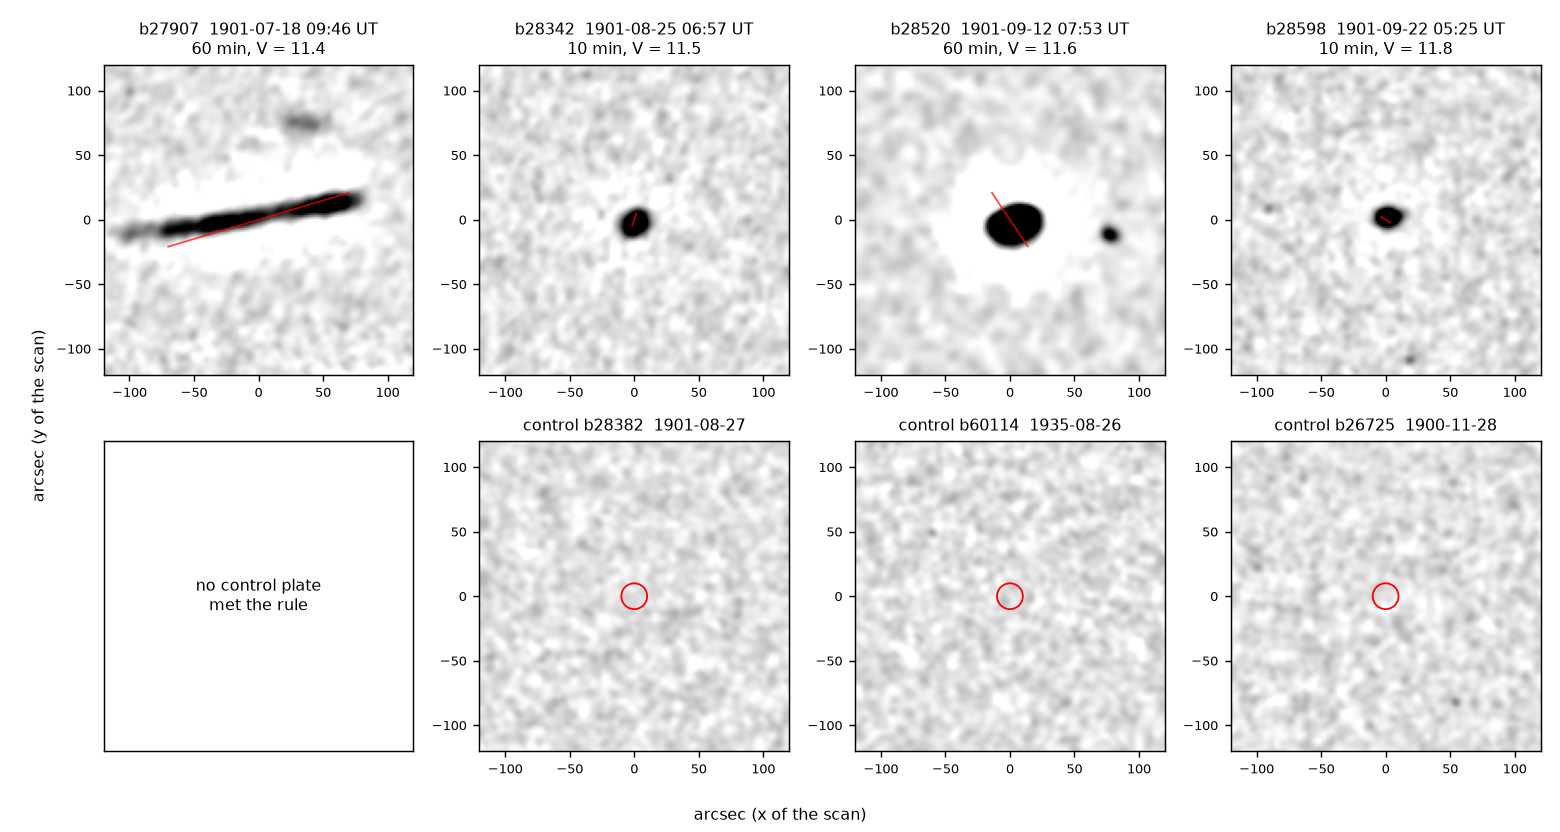
\includegraphics[width=\textwidth]{fig_ivar.png}
\caption{Top: the four passing 1901 plates. Each panel is the noise-normalised image $z$, 240\as{} wide, centred on the predicted midpoint position after the registered refit. The red line is the predicted motion of Ivar during the exposure. Bottom: the first control plate of another date at the same sky position (DASCH WCS; the red circle has a radius of 10\as). b27907 has no control plate. Axes in arcseconds along the scan axes.}
\label{fig:stamps}
\end{figure}

\section{Controls}
\begin{itemize}
\item \emph{Plates of other dates.} Table~\ref{tab:ctrl} gives the maximum $z$ within 5\as{} of the Ivar position. On the six control plates the values are 0.33 to 1.19. On the three target plates they are 31.9 to 62.7. A star or a permanent flaw of the scan at these positions would show on the control plates. Figure~\ref{fig:stamps} (bottom row) shows one control plate for each position.
\item \emph{Catalogued stars.} The nearest ATLAS star brighter than magnitude 16 is 81.7\as{} (b27907), 33.0\as{} (b28342), 320\as{} (b28520) and 152\as{} (b28598) from the predicted position. The verification stage found no catalogued star brighter than magnitude 19 within 20\as{} of a predicted position.
\item \emph{Known objects.} SkyBoT returns only (1627) Ivar within 180\as{} of the four positions. The next object is (7388) Marcomorelli, $V=18.7$, at 254\as{} on b27907. SkyBoT puts Ivar 23.3\as, 32.6\as, 19.2\as{} and 26.5\as{} from the Horizons position. The cause of this difference (a time scale or the precision of the SkyBoT ephemeris) is not known. It does not change the test, which uses the Horizons track.
\item \emph{Ephemeris and site.} A fresh Horizons query (solution JPL\#1545) gives the predicted positions again to 0.0\as. For the four 1901 plates, the Cambridge (site 802) position is 20\as{} to 34\as{} from the Arequipa position, and the geocentric position is 5\as{} to 14\as{} from it. The sources are within about 4\as{} of the Arequipa position on three plates (next section). This agrees with the assumed site.
\end{itemize}

\begin{table}[h]
\centering\small
\begin{tabular}{lrll}\toprule
Target plate & max $z$ (5\as) & Control plates (date, max $z$) \\\midrule
b27907 & 17.0 & none met the rule \\
b28342 & 31.9 & b28382 (1901-08-27, 0.71), b26726 (1900-11-28, 0.33) \\
b28520 & 62.7 & b60114 (1935-08-26, 0.90), b60155 (1935-09-03, 0.66) \\
b28598 & 42.8 & b26725 (1900-11-28, 0.76), b26524 (1900-11-10, 1.19) \\\bottomrule
\end{tabular}
\caption{Plates of other dates at the same sky position (\texttt{data/controls.json}).}
\label{tab:ctrl}
\end{table}

\section{Measurements after the decision}
Table~\ref{tab:post} gives the results of \texttt{src/posthoc.py}.
\begin{itemize}
\item \emph{Position.} On b28342, b28520 and b28598 the centroid of the source is 0.7\as, 3.1\as{} and 4.0\as{} from the predicted midpoint position. The peak pixels of the registered statistic are 4.0\as, 2.5\as{} and 0.5\as{} from it. We give the agreement as ``within about 4\as''. These values are not astrometry: the reference frame is the DASCH WCS with a median star offset, and on b28342 no star matched, so the DASCH WCS is used without correction. Ivar moves about 50\as{} to 60\as{} per hour on these dates, so an error of a few minutes in a DASCH midpoint gives a few arcseconds of offset.
\item \emph{The trail on b27907.} The source is a connected region 162\as{} long with an axis ratio of 12. Its long axis is $7^\circ$ from the predicted direction of motion. The predicted trail for the 60-min exposure is 146\as. Along the predicted track, $z$ is 10 or more from $-0.50$\,h to $+0.42$\,h and below 10 at all other track points within $\pm1$\,h (\texttt{data/posthoc.json}). The signal thus starts and ends near the predicted positions at the start and the end of the exposure. A fixed star does not give this shape. In Figure~\ref{fig:stamps} the trail extends past the predicted segment at its left end. We did not measure the cause.
\item \emph{Other shapes.} On the two 10-min plates the predicted trail (10\as{} and 8\as) is shorter than the image size (25\as{} and 19\as), so the shape does not test the motion. On the 60-min plate b28520 the predicted trail is 50\as, but the source is 42\as{} long with an axis ratio of 1.5, and its long axis is $72^\circ$ from the direction of motion. Along the track, $z$ is 10 or more from $-0.33$\,h to $+0.58$\,h, which is longer than the 60-min exposure. We did not find the cause of this shape. It is a reason for an examination of the plate.
\item \emph{Brightness.} The expected photographic magnitude is about $V+0.8$, that is 12.4 on b28520 and 12.6 on b28598. The fit of ATLAS magnitudes gives 12.3 (rms of the fit 0.53) and 11.8 (rms 0.65). On b27907 the estimate is 13.3 with rms 1.56, for a trailed source. On b28342 no star matched, so there is no estimate. The magnitude band of the plates is not calibrated here, so this check is approximate.
\end{itemize}

\begin{table}[h]
\centering\small
\begin{tabular}{lrrrrrl}\toprule
Plate & peak $z$ & centroid (\as) & length (\as) & axis ratio & angle to motion & $z\ge10$ on track (h) \\\midrule
b27907 & 27.1 & -- & 162 (pred.\ 146) & 12.0 & $7^\circ$ & $-0.50$ to $+0.42$ \\
b28342 & 30.0 & 0.7 & 25 (pred.\ 10) & 1.2 & $31^\circ$ & $-0.25$ to $+0.25$ \\
b28520 & 73.0 & 3.1 & 42 (pred.\ 50) & 1.5 & $72^\circ$ & $-0.33$ to $+0.58$ \\
b28598 & 40.8 & 4.0 & 19 (pred.\ 8) & 1.3 & $38^\circ$ & $-0.33$ to $+0.25$ \\\bottomrule
\end{tabular}
\caption{Measurements after the decision (\texttt{data/posthoc.json}). Peak $z$: within 40\as{} of the predicted midpoint position. Centroid: offset from that position (b27907 is a trail, so a centroid offset from the midpoint has no meaning). Length: extent of the connected source region; pred.: predicted trail length. The last column uses the maximum $z$ within 6\as{} of each 5-min track point.}
\label{tab:post}
\end{table}

\section{How the results were checked}
\begin{itemize}
\item \texttt{checks/rerun.py} downloads the six registered cutouts, the ATLAS stars, the six control cutouts, the control plate lists, the Horizons positions and the SkyBoT lists again into a new directory. It reruns the registered test, the controls, the $P_{\rm null}$ bounds and the measurements after the decision, and compares every number of this paper with \texttt{data/expected.json}. The plate list and the predictions are fixed registered inputs; the script does not rerun the plate selection. \texttt{checks/ci.sh} runs it with pinned packages and reports whether the new cutouts are byte-identical to the ones used here.
\item In the verification stage, the solve-stage rerun printed ``OK'' from a clean clone, with the committed cutouts and with a fresh download. The five fresh cutouts were byte-identical to the committed ones. A rerun of the control script gave an identical output file.
\item The verification stage checked the plate selection against the rule on the 25 candidate plates, checked the SBDB and MPC records, and wrote the independent measurement code that is now \texttt{src/posthoc.py}.
\end{itemize}

\section{Limits}
\begin{itemize}
\item The identification uses the plate scans only. Nobody examined the glass plates or the observing logs. No person looked at the images; Figure~\ref{fig:stamps} was made in the write stage and was examined only by the AI model that wrote this text.
\item No astrometry in MPC format was measured, and no position was reported to the MPC. The positions in Table~\ref{tab:post} are offsets in the DASCH WCS frame.
\item The record date rests on b27907, which is weak alone in the registered test ($p_0=0.243$) and has no control plate. Its main support is the trail shape, a check made after the result.
\item The source on b28520 is not elongated along the predicted motion, and its track profile is longer than the exposure. The cause is not known.
\item $P_{\rm null}$ is a product of four rates, each from 300 regions. We give it as about $10^{-6}$, with a bound of $1.8\times10^{-5}$.
\item No injection test ran for Ivar. The positive control of the method is the Ganymed result~\cite{wu2026ganymed}, with the same code.
\item The Arequipa site of the b series and the DASCH midpoints and exposure times are taken as correct. The ephemeris has one source (Horizons, solution JPL\#1545).
\item The plate selection depends on DASCH metadata. The 1906 apparition gave no candidate plate, and the single 1929 plate fails. Plates outside the rule, for example b plates of 1901 with a shallower limit, were not searched.
\item ``Earliest known image'' rests on the SBDB, the MPC list and the searches of Section~1. There is no complete survey of plate archives.
\end{itemize}

\section*{Data and code}
The result folder has the protocol (\texttt{PROTOCOL.md}), the code (\texttt{src/}), the registered inputs and results (\texttt{data/}), the expected values (\texttt{data/expected.json}), the list of numbers and their sources (\texttt{NUMBERS.md}), and \texttt{checks/ci.sh}, which reruns everything from the public data.

\section*{Acknowledgements}
This research uses data from DASCH (Digital Access to a Sky Century @ Harvard); we thank the DASCH project and the Harvard plate stacks. Ephemerides are from the JPL Horizons system and the JPL Small-Body Database. This work made use of the IMCCE SkyBoT service.

\begin{thebibliography}{12}
\bibitem{sbdb} JPL Small-Body Database, (1627) Ivar, \url{https://ssd.jpl.nasa.gov/tools/sbdb_lookup.html#/?sstr=1627}; API \url{https://ssd-api.jpl.nasa.gov/sbdb.api?sstr=1627&discovery=1&phys-par=1}. Accessed 2026 Nov 28.
\bibitem{mpcobs} Minor Planet Center, observations of (1627), \texttt{get-obs} API, \url{https://data.minorplanetcenter.net/api/get-obs} (designation 1627, format OBS80). Accessed 2026 Nov 28.
\bibitem{wiki} Wikipedia, ``1627 Ivar'', \url{https://en.wikipedia.org/wiki/1627_Ivar}. Accessed 2026 Nov 28.
\bibitem{horizons} JPL Horizons system, \url{https://ssd.jpl.nasa.gov/horizons/}; API \url{https://ssd.jpl.nasa.gov/api/horizons.api}. Accessed 2026 Nov 28.
\bibitem{dasch} DASCH Data Release 7, Harvard College Observatory, \url{https://dasch.cfa.harvard.edu/dr7/}. Accessed 2026 Nov 28.
\bibitem{grindlay2012} J.~Grindlay, S.~Tang, E.~Los, M.~Servillat, ``Opening the 100-Year Window for Time-Domain Astronomy'', Proc.\ IAU 7 (S285), 29--34 (2011), doi:\href{https://doi.org/10.1017/S1743921312000166}{10.1017/S1743921312000166}.
\bibitem{tonry2018} J.\,L.~Tonry, L.~Denneau, H.~Flewelling, A.\,N.~Heinze, et al., ``The ATLAS All-Sky Stellar Reference Catalog'', ApJ 867, 105 (2018), doi:\href{https://doi.org/10.3847/1538-4357/aae386}{10.3847/1538-4357/aae386}.
\bibitem{skybot} IMCCE, SkyBoT cone search service, \url{https://ssp.imcce.fr/webservices/skybot/}. Accessed 2026 Nov 28.
\bibitem{murtagh2026} J.~Murtagh, C.\,O.~Chandler, M.~Juri\'c, et al., ``A Century-Long Archival Search and Analysis of the Rubin Observatory-Discovered Dwarf Planet Candidate 2026 ED$_{138}$'', arXiv:\href{https://arxiv.org/abs/2611.02371}{2611.02371} (2026).
\bibitem{graham2026} P.~Graham, ``Candidate images of Pluto on archival plates from 1908 and 1909'' (2026), \url{https://github.com/6/clank-lab/tree/main/results/pluto-prediscovery}, doi:\href{https://doi.org/10.5281/zenodo.24387450}{10.5281/zenodo.24387450}.
\bibitem{wu2026metcalf} Q.~Wu, ``A systematic time error in the DASCH metadata of J.\,H.~Metcalf's early `ma' plates, and Pluto on four Harvard plates of 1908 and 1909'' (2026), doi:\href{https://doi.org/10.5281/zenodo.24523190}{10.5281/zenodo.24523190}.
\bibitem{wu2026ganymed} Q.~Wu, ``(1036) Ganymed on Harvard plates of 1898, 26 years before its discovery, and a candidate image of (624) Hektor from 1901'' (2026), doi:\href{https://doi.org/10.5281/zenodo.24600765}{10.5281/zenodo.24600765}.
\end{thebibliography}
\end{document}
